\newpage
\subsection{Caso d'uso UC5: Recupero password}
\label{UC5}
\begin{figure}[ht]
	\centering
	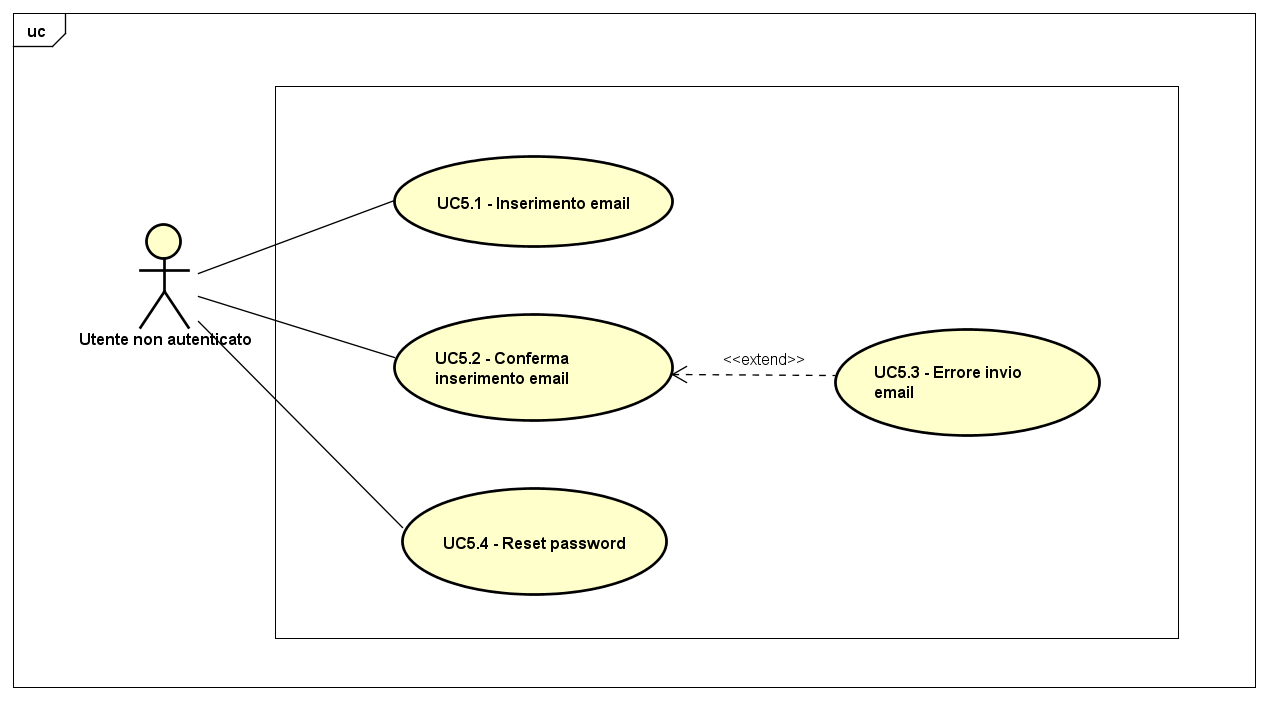
\includegraphics[scale=0.45]{UML/UC5.png}
	\caption{UC5: Recupero password}
\end{figure}

\begin{longtable}{ l | p{11cm}}
	\hline
	\rowcolor{Gray}
	 \multicolumn{2}{c}{UC5 - Recupero password} \\
	 \hline
	\textbf{Attori} & Utente non autenticato \\
	\textbf{Descrizione} & L'attore recupera la password del proprio account API Market tramite l'invio di una email \\
	\textbf{Pre-Condizioni} & L'attore ha scelto di recuperare la password del proprio account API Market. L'applicazione visualizza le pagine preposte agli utenti non autenticati. \\
	\textbf{Post-Condizioni} & L'attore ha ricevuto nella propria casella email un link per resettare la password del proprio account API Market, oppure la procedura è fallita \\
	\textbf{Scenario Principale} & 
	\begin{enumerate*}[label=(\arabic*.),itemjoin={\newline}]
		\item L'attore può inserire la propria email (UC5.1)
		\item L'attore può confermare l'indirizzo email inserito, al quale l'applicazione web invierà un link per resettare la password (UC5.2)
		\item L'attore, se ha richiesto il recupero della password ed ha aperto il link per poterla resettare, può effettuare il reset password in una apposita schermata (UC5.4)
	\end{enumerate*}\\
	\textbf{Scenari Alternativi} & 
	\begin{enumerate*}[label=(\arabic*.),itemjoin={\newline}]
		\item L'attore, dopo aver confermato l'invio della email di reset password, se ha inserito un'email non valida o inesistente, può visualizzare un messaggio d'errore e l'email di reset password non viene inviata (UC5.3)
	\end{enumerate*}\\
\end{longtable}

\subsubsection{Caso d'uso UC5.1: Inserimento email}
\label{UC5_1}

\begin{minipage}{\linewidth}
\begin{longtable}{ l | p{11cm}}
	\hline
	\rowcolor{Gray}
	 \multicolumn{2}{c}{UC5.1 - Inserimento email} \\
	 \hline
	\textbf{Attori} & Utente non autenticato \\
	\textbf{Descrizione} & L'attore inserisce la sua email \\
	\textbf{Pre-Condizioni} & L'attore ha dimenticato la password e l'applicazione web mostra la schermata di recupero password \\
	\textbf{Post-Condizioni} & L'attore ha inserito l'email relativa all'account di cui desidera recuperare la password \\
	\textbf{Scenario Principale} & \begin{enumerate*}[label=(\arabic*.),itemjoin={\newline}]
		\item L'attore può inserire la propria email (UC5.1)
	\end{enumerate*}\\
\end{longtable}
\end{minipage}

\subsubsection{Caso d'uso UC5.2: Conferma inserimento email}
\label{UC5_2}

\begin{minipage}{\linewidth}
\begin{longtable}{ l | p{11cm}}
	\hline
	\rowcolor{Gray}
	 \multicolumn{2}{c}{UC5.2 - Conferma inserimento email} \\
	 \hline
	\textbf{Attori} & Utente non autenticato \\
	\textbf{Descrizione} & L'attore conferma l'inserimento del proprio indirizzo email tramite un apposito pulsante \\
	\textbf{Pre-Condizioni} & L'attore ha inserito l'email dell'account di cui intende recuperare la password \\
	\textbf{Post-Condizioni} & L'attore ha confermato i dati immessi, visualizzando un messaggio di successo e ricevendo tramite mail il link di reset password \\
	\textbf{Scenario Principale} & \begin{enumerate*}[label=(\arabic*.),itemjoin={\newline}]
		\item L'attore può confermare i dati immessi, visualizzando un messaggio di successo e ricevendo tramite email il link per resettare la password (UC5.4) e viene reindirizzato alla schermata principale (UC1)
	\end{enumerate*}\\
	\textbf{Scenari Alternativi} & 
	\begin{enumerate*}[label=(\arabic*.),itemjoin={\newline}]
		\item L'attore ha inserito un'email non valida o inesistente, visualizza un messaggio d'errore e l'email di reset password non avviene (UC5.3)
	\end{enumerate*}\\
\end{longtable}
\end{minipage}

\subsubsection{Caso d'uso UC5.3: Errore invio email}
\label{UC5_3}

\begin{minipage}{\linewidth}
\begin{longtable}{ l | p{11cm}}
	\hline
	\rowcolor{Gray}
	 \multicolumn{2}{c}{UC5.3 - Errore invio email} \\
	 \hline
	\textbf{Attori} & Utente non autenticato \\
	\textbf{Descrizione} & L'attore riceve un messaggio di errore dovuto all'inserimento di un'email non valida o inesistente \\
	\textbf{Pre-Condizioni} & L'attore ha dimenticato la password e ha inserito l'email per poterla recuperare \\
	\textbf{Post-Condizioni} & L'attore riceve un messaggio di errore e può eventualmente ripetere la procedura di recupero password \\
	\textbf{Scenario Principale} & \begin{enumerate*}[label=(\arabic*.),itemjoin={\newline}]
		\item L'attore visualizza un messaggio d'errore per aver lasciato il campo vuoto o per aver inserito un indirizzo inesistente. Può ripetere la procedura (UC5)
	\end{enumerate*}\\
\end{longtable}
\end{minipage}

\newpage
\subsubsection{Caso d'uso UC5.4: Reset password}
\label{UC5_4}
\begin{figure}[ht]
	\centering
	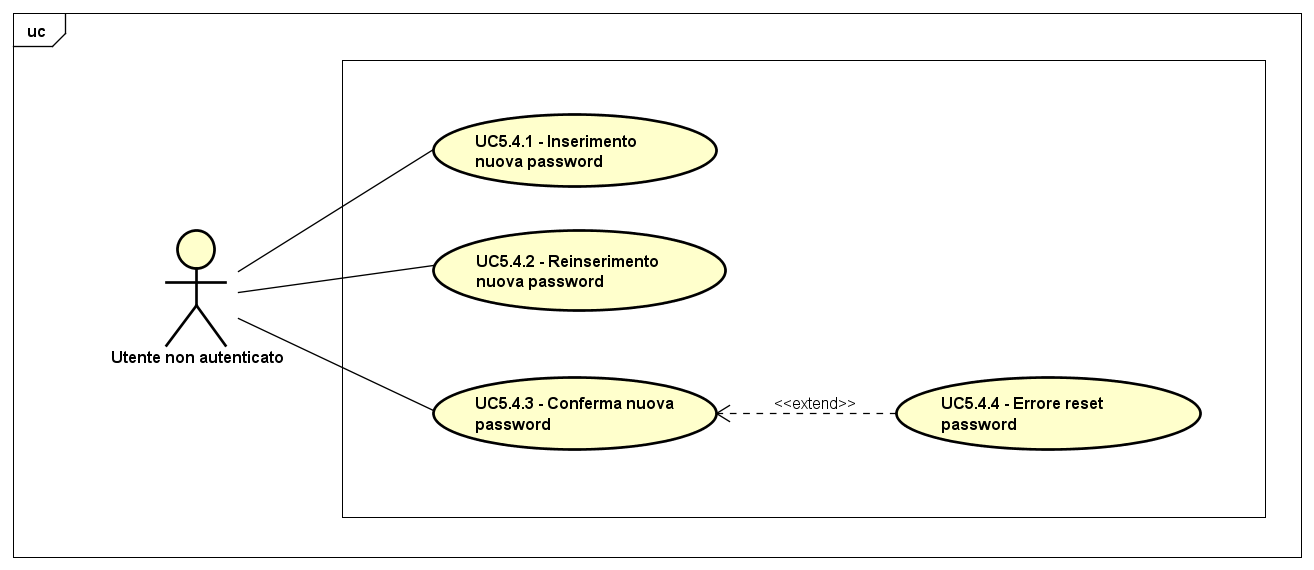
\includegraphics[scale=0.45]{UML/UC5_4.png}
	\caption{UC5.4: Reset password}
\end{figure}

\begin{minipage}{\linewidth}
	\begin{longtable}{ l | p{11cm}}
		\hline
		\rowcolor{Gray}
		\multicolumn{2}{c}{UC5.4 - Reset password} \\
		\hline
		\textbf{Attori} & Utente non autenticato \\
		\textbf{Descrizione} & L'attore ha ricevuto un link per la schermata di reset della propria password \\
		\textbf{Pre-Condizioni} & L'attore ha richiesto il recupero della password ed ha aperto il link per poterla resettare \\
		\textbf{Post-Condizioni} & L'attore ha resettato con successo la password \\
		\textbf{Scenario Principale} & 
		\begin{enumerate*}[label=(\arabic*.),itemjoin={\newline}]
			\item L'attore può inserire la nuova password desiderata (UC5.4.1)
			\item L'attore può reinserire la nuova password desiderata (UC5.4.2)
			\item L'attore può confermare i dati inseriti e completare la procedura con successo (UC5.4.3)
		\end{enumerate*}\\
		\textbf{Scenari Alternativi} & 
		\begin{enumerate*}[label=(\arabic*.),itemjoin={\newline}]
			\item L'attore, dopo aver confermato i dati inseriti, se le password inserite non coincidono o i campi risultano vuoti, può visualizzare un errore (UC5.4.4)
		\end{enumerate*}\\
	\end{longtable}
\end{minipage}

\paragraph{Caso d'uso UC5.4.1: Inserimento nuova password}
\label{UC5_4_1}

\begin{minipage}{\linewidth}
	\begin{longtable}{ l | p{11cm}}
		\hline
		\rowcolor{Gray}
		\multicolumn{2}{c}{UC5.4.1 - Inserimento nuova password} \\
		\hline
		\textbf{Attori} & Utente non autenticato \\
		\textbf{Descrizione} & L'attore inserisce la nuova password per il proprio account \\
		\textbf{Pre-Condizioni} & L'applicazione mostra la schermata di reset password \\
		\textbf{Post-Condizioni} & L'attore ha inserito la nuova password \\
		\textbf{Scenario Principale} & 
		\begin{enumerate*}[label=(\arabic*.),itemjoin={\newline}]
			\item L'attore può inserire la nuova password per il proprio account
		\end{enumerate*}\\
	\end{longtable}
\end{minipage}

\paragraph{Caso d'uso UC5.4.2: Reinserimento nuova password}
\label{UC5_4_2}

\begin{minipage}{\linewidth}
	\begin{longtable}{ l | p{11cm}}
		\hline
		\rowcolor{Gray}
		\multicolumn{2}{c}{UC5.4.2 - Reinserimento nuova password} \\
		\hline
		\textbf{Attori} & Utente non autenticato \\
		\textbf{Descrizione} & L'attore reinserisce la nuova password per il proprio account \\
		\textbf{Pre-Condizioni} & L'applicazione mostra la schermata di reset password \\
		\textbf{Post-Condizioni} & L'attore ha reinserito la nuova password \\
		\textbf{Scenario Principale} & 
		\begin{enumerate*}[label=(\arabic*.),itemjoin={\newline}]
			\item L'attore può reinserire la nuova password per il proprio account
		\end{enumerate*}\\
	\end{longtable}
\end{minipage}

\paragraph{Caso d'uso UC5.4.3: Conferma nuova password}
\label{UC5_4_3}

\begin{minipage}{\linewidth}
	\begin{longtable}{ l | p{11cm}}
		\hline
		\rowcolor{Gray}
		\multicolumn{2}{c}{UC5.4.3 - Conferma nuova password} \\
		\hline
		\textbf{Attori} & Utente non autenticato \\
		\textbf{Descrizione} & L'attore conferma i dati inseriti per poter resettare la propria password \\
		\textbf{Pre-Condizioni} & L'applicazione mostra la schermata di reset password \\
		\textbf{Post-Condizioni} & L'attore ha confermato i nuovi dati per il proprio account \\
		\textbf{Scenario Principale} & 
		\begin{enumerate*}[label=(\arabic*.),itemjoin={\newline}]
			\item L'attore può confermare i nuovi dati per il proprio account, visualizzando un messaggio di successo e venendo reindirizzato alla schermata principale (UC1)
		\end{enumerate*}\\
	\end{longtable}
\end{minipage}

\paragraph{Caso d'uso UC5.4.4: Errore reset password}
\label{UC5_4_4}

\begin{minipage}{\linewidth}
	\begin{longtable}{ l | p{11cm}}
		\hline
		\rowcolor{Gray}
		\multicolumn{2}{c}{UC5.4.4 - Errore reset password} \\
		\hline
		\textbf{Attori} & Utente non autenticato \\
		\textbf{Descrizione} & L'attore conferma i dati inseriti per poter resettare la propria password \\
		\textbf{Pre-Condizioni} & L'attore ha confermato i dati inseriti per poter resettare la propria password \\
		\textbf{Post-Condizioni} & L'attore non ha confermato con successo i propri nuovi dati di accesso \\
		\textbf{Scenario Principale} & 
		\begin{enumerate*}[label=(\arabic*.),itemjoin={\newline}]
			\item L'attore visualizza un messaggio di errore poiché le password non coincidono o i campi sono vuoti
		\end{enumerate*}\\
	\end{longtable}
\end{minipage}